% THIS IS SIGPROC-SP.TEX - VERSION 3.1
% WORKS WITH V3.2SP OF ACM_PROC_ARTICLE-SP.CLS
% APRIL 2009
%
% It is an example file showing how to use the 'acm_proc_article-sp.cls' V3.2SP
% LaTeX2e document class file for Conference Proceedings submissions.
% ----------------------------------------------------------------------------------------------------------------
% This .tex file (and associated .cls V3.2SP) *DOES NOT* produce:
%       1) The Permission Statement
%       2) The Conference (location) Info information
%       3) The Copyright Line with ACM data
%       4) Page numbering
% ---------------------------------------------------------------------------------------------------------------
% It is an example which *does* use the .bib file (from which the .bbl file
% is produced).
% REMEMBER HOWEVER: After having produced the .bbl file,
% and prior to final submission,
% you need to 'insert'  your .bbl file into your source .tex file so as to provide
% ONE 'self-contained' source file.
%
% Questions regarding SIGS should be sent to
% Adrienne Griscti ---> griscti@acm.org
%
% Questions/suggestions regarding the guidelines, .tex and .cls files, etc. to
% Gerald Murray ---> murray@hq.acm.org
%
% For tracking purposes - this is V3.1SP - APRIL 2009

%\documentclass{acm_proc_article-sp}  % mise en comment (19/01/2016)

\documentclass{sig-alternate-05-2015} % ajout (19/01/2016)

%%%\CopyrightYear{2016}
\setcopyright{acmlicensed}
\conferenceinfo{HSCC'17,}{April 17--20, 2017, Pittsburgh, Pennsylvania}
%\isbn{978-1-4503-3955-1/16/04}\acmPrice{\$15.00}
\doi{http://dx.doi.org/XXXX.XXXX}

%Authors, replace the red X's with your assigned DOI string.

\clubpenalty=10000
\widowpenalty = 10000


\usepackage{listings}
\usepackage{graphicx} % Required for including pictures
\usepackage{amsfonts}
\usepackage{amsmath}

\usepackage{tikz}
\usepgflibrary{plotmarks}
\usepgfmodule[plot]
\usepackage{pgfplots}
\usepackage{cite}
\usepackage{epsfig}
\usepackage{float} % Allows putting an [H] in \begin{figure} to specify the exact location of the figure
\usepackage{wrapfig} % Allows in-line images such as the example fish picture
%\usepackage{amsthm}
\usepackage{amssymb}
\usepackage{hyperref}
\usepackage{tikz}
\usepackage{multirow}
\usepackage{comment}
\usepackage[]{algorithm2e}
\usepackage{caption}
\usepackage{subcaption}
\usepackage{url}
% \font\dsrom=dsrom10 scaled 1200
% \def \ind{\textrm{\dsrom{1}}}

 \newcommand\ForAuthors[1]%          %  temporary remark for the
 {\par\smallskip                     %  authors:
  \begin{center}%                    %
   \fbox%                            %    --------
   {\parbox{0.9\linewidth}%          %    |  #1  |
    {\raggedright\sc--- #1}%         %    --------
   }%                                %
  \end{center}%                      %
  \par\smallskip                     %
 }        


\newcommand{\comm}[1]{}
\newtheorem{definition}{Definition}
\newtheorem{theorem}{Theorem}
\newtheorem{proposition}{Proposition}
\newtheorem{lemma}{Lemma}
\newtheorem{example}{Example}

\def\N{{\mathbb N}}
\def\Z{{\mathbb Z}}
\def\R{{\mathbb R}}
\def\int#1{\mbox{$[ #1 ]$}}

\newcommand{\IR}{\mathbb{IR}}
\newcommand{\va}{{\bf a}}
\newcommand{\vb}{{\bf b}}
\newcommand{\vc}{{\bf c}}
\newcommand{\vd}{{\bf d}}
\newcommand{\vf}{{\bf f}}
\newcommand{\vh}{{\bf h}}
\newcommand{\vg}{{\bf g}}
\newcommand{\vm}{{\bf m}}
\newcommand{\vu}{{\bf u}}
\newcommand{\vv}{{\bf v}}
\newcommand{\vx}{{\bf x}}
\newcommand{\vy}{{\bf y}}
\newcommand{\vt}{{\bf t}}
\newcommand{\vz}{{\bf z}}
\newcommand{\vJ}{{\bf J}}
\newcommand{\vA}{{\bf A}}
\newcommand{\vB}{{\bf B}}
\DeclareMathOperator{\interior}{int}
\newcommand{\inter}[1]{\left[#1\right]}
\DeclareMathOperator{\diag}{Diag}
\DeclareMathOperator{\offdiag}{OffDiag}
\DeclareMathOperator{\range}{range}
\usepackage{color}

\newcommand{\dual}{\mbox{dual }}
\newcommand{\pro}{\mbox{pro }}
\newcommand{\semb}{[ \! [}
\newcommand{\seme}{] \! ]}
%\newcommand{\comment2}[1]{}
\newcommand{\norma}[1]{\mbox{$\mid \! \mid #1 \mid \! \mid^a$}}
\newcommand{\normu}[1]{\mbox{$\mid \! \mid #1 \mid \! \mid^\cup$}}
\newcommand{\normn}[1]{\mbox{$\mid \! \mid #1 \mid \! \mid^\cap$}}
\newtheorem{sketch}{Sketch of proof.}
\newtheorem{problem}{Problem}
\newtheorem{property}{Property}
\def\ve{\vec{\varepsilon}}
\def\vp{\vec{\varphi}}
\def\ua{\uparrow_\circ}
\def\da{\downarrow_\circ}
\def\ra{\rightarrow}
\def\bbr{{\Bbb R}}
\def\bbf{{\Bbb F}}
\def\F{{\Bbb F}}
\def\A{{\Bbb A}}
\def\calD{{\Bbb D}}
\def\I{{\Bbb I \Bbb R}}
\def\K{{\Bbb I \Bbb K}}
%\def\RAff{{\Bbb R \Bbb A}}
\def\RAff{{\Bbb A \Bbb R}}
%\def\IAff{{\Bbb I \Bbb A}}
\def\IAff{{\Bbb A \Bbb I}}

\makeatletter
\newcommand\listofTODO{\section*{Remaining TODO}\@starttoc{tdo}}
\makeatother
\newcommand{\addTODO}[1]{\addcontentsline{tdo}{toc}{#1}}
\newcommand{\TODO}[1]{{\bf{\scriptsize #1}\addTODO{#1}}}
\newcommand{\SP}[1]{\TODO{Sylvie : #1}}
\newcommand{\EG}[1]{\TODO{Eric : #1}}

\definecolor{cof}{RGB}{219,144,71}
\definecolor{pur}{RGB}{186,146,162}
\definecolor{greeo}{RGB}{91,173,69}
\definecolor{greet}{RGB}{52,111,72}
\definecolor{red}{RGB}{210,0,32}

%\theoremstyle{remark}
\newtheorem{remark}{Remark}
\def\norm#1{\mbox{$\left\| #1 \right\|_1$}} 


\usetikzlibrary{positioning}
\tikzset{main node/.style={circle,fill=blue!20,draw,minimum size=0.8cm,inner sep=0pt},
            }

\begin{document}

\def\transpose#1{{}^t \! #1}
% boldface letters for intervals
\def\bfm#1{\protect{\makebox{\boldmath $#1$}}}
\def\a {\bfm{a}}
\def\b {\bfm{b}}
\def\c {\bfm{c}}
\def\d {\bfm{d}}
\def\e {\bfm{e}}
\def\f {\bfm{f}}
\def\g {\bfm{g}}
\def\h {\bfm{h}}
\def\ii {\bfm{i}}       % \i is already 'i without dot'
\def\j {\bfm{j}}
\def\k {\bfm{k}}
\def\l {\bfm{l}}
\def\m {\bfm{m}}
\def\n {\bfm{n}}
\def\o {\bfm{o}}
\def\p {\bfm{p}}
\def\q {\bfm{q}}
\def\r {\bfm{r}}
\def\s {\bfm{s}}
\def\t {\bfm{t}}
\def\u {\bfm{u}}
\def\vv {\bfm{v}}       % \v is already 'check' 
\def\w {\bfm{w}}
\def\x {\bfm{x}}
\def\y {\bfm{y}}
\def\z {\bfm{z}}
%\def\A {\bfm{A}}
\def\B {\bfm{B}}
\def\C {\bfm{C}}
\def\DD{\bfm{D}}        % \D is already \displaystyle
\def\E {\bfm{E}}
%\def\F {\bfm{F}}
\def\G {\bfm{G}}
\def\H {\bfm{H}}
%\def\I {\bfm{I}}
\def\J {\bfm{J}}
%\def\K {\bfm{K}}
\def\L {\bfm{L}}
\def\M {\bfm{M}}
\def\N {\bfm{N}}
\def\O {\bfm{O}}
\def\P {\bfm{P}}
\def\Q {\bfm{Q}}
%\def\R {\bfm{R}}
\def\S {\bfm{S}}
\def\T {\bfm{T}}
\def\U {\bfm{U}}
\def\V {\bfm{V}}
\def\W {\bfm{W}}
\def\X {\bfm{X}}
\def\Y {\bfm{Y}}


\title{Forward inner-approximated reachability  of non-linear continuous systems}
%\subtitle{[Extended Abstract]
%\titlenote{A full version of this paper is available as
%\textit{Author's Guide to Preparing ACM SIG Proceedings Using
%\LaTeX$2_\epsilon$\ and BibTeX} at
%\texttt{www.acm.org/eaddress.htm}}}
%
% You need the command \numberofauthors to handle the 'placement
% and alignment' of the authors beneath the title.
%
% For aesthetic reasons, we recommend 'three authors at a time'
% i.e. three 'name/affiliation blocks' be placed beneath the title.
%
% NOTE: You are NOT restricted in how many 'rows' of
% "name/affiliations" may appear. We just ask that you restrict
% the number of 'columns' to three.
%
% Because of the available 'opening page real-estate'
% we ask you to refrain from putting more than six authors
% (two rows with three columns) beneath the article title.
% More than six makes the first-page appear very cluttered indeed.
%
% Use the \alignauthor commands to handle the names
% and affiliations for an 'aesthetic maximum' of six authors.
% Add names, affiliations, addresses for
% the seventh etc. author(s) as the argument for the
% \additionalauthors command.
% These 'additional authors' will be output/set for you
% without further effort on your part as the last section in
% the body of your article BEFORE References or any Appendices.

\numberofauthors{2} %  in this sample file, there are a *total*
% of EIGHT authors. SIX appear on the 'first-page' (for formatting
% reasons) and the remaining two appear in the \additionalauthors section.
%
%\author{
% You can go ahead and credit any number of authors here,
% e.g. one 'row of three' or two rows (consisting of one row of three
% and a second row of one, two or three).
%
% The command \alignauthor (no curly braces needed) should
% precede each author name, affiliation/snail-mail address and
% e-mail address. Additionally, tag each line of
% affiliation/address with \affaddr, and tag the
% e-mail address with \email.
%
% 1st. author
%\alignauthor E. Goubault \\ %\titlenote{Dr.~Trovato insisted his name be first.}\\
%       \affaddr{LIX, Ecole Polytechnique, CNRS, }\\
%       \affaddr{Universit\'e Paris-Saclay, 91128 Palaiseau, France} \\
%       \email{\small goubault@lix.polytechnique.fr}
% 2nd. author
%\alignauthor S. Putot \\ %\titlenote{The secretary disavows
%any knowledge of this author's actions.}\\
%       \affaddr{LIX, Ecole Polytechnique, CNRS, } \\
%       \affaddr{Universit\'e Paris-Saclay, 91128 Palaiseau, France}\\
%       \affaddr{France}\\
%       \email{\small putot@lix.polytechnique.fr}
%}
\author{}

\maketitle
\begin{abstract}
We propose an approach for computing inner-approximations (also called under-approximations) of reachable sets of dynamical systems 
defined by non-linear, uncertain, ordinary differential equations. This is a notoriously difficult problem, much more intricate than 
outer-approximations for whi\-ch there exist well known solutions, mostly based on Taylor models. 
The few methods developped recently for inner-approximation mostly rely on backward flowmaps, and extra ingredients, either coming from optimisation, 
or involving topological criteria, are required. Our solution, in comparison, builds on rather inexpensive set-based methods, namely a generalized
mean-value theorem combined with Taylor models outer-approximations (also called over-approx\-imations) of the flow and its jacobian with respect 
to the uncertain inputs and parameters.
%for inner-approximations is also based on Taylor models, but contrarily to the few methods developped recently, 
% is a direct forward method, which only relies on rather inexpensive set-based methods, namely a generalized mean-value theorem 
%applied to 
% instead of the %clever, but still complicated, 
%existing  methods relying on backward flowmaps and for which extra ingredients, either coming from optimisation, or involving topological criteria, are required. 
We are able to show with our prototype Matlab implementation that our method is both efficient and
precise on classical examples. 
%\ForAuthors{Est-ce dangereux de se placer un peu sur la complexite? On pourrait nous reprocher d'avoir un
%nombre d'equations en le produit du nombre d'equations d'origine, avec le nombre de variables... Mais la methode
%de Sriram et celle des chinois est potentiellement tres complexe.}
%Our method, being based on Taylor models and being a forward method, also provides outer-approximations, naturally. 
The combination of such forward inner and outer Taylor-model based approximations 
can be used as a basis for the verification and falsification of properties
of cyber-physical systems. 
%- forward inner- and outer- approximations 
%of the set of  states reachable by an uncertain hybrid systems, that is with uncertain initial conditions and parameters.\\
%- little studied and difficult problem, the small number of existing approaches mostly attack the dual problem aof backward inner-apporximated reachability \\
%- based on a combination of Taylor based methids for teh solution of IVP and generalized mean value theorem for inner-approximation~\cite{hscc14}\\
%- experiments with matlab implementation
\end{abstract}

% A category with the (minimum) three required fields
% CATEGORIES A VERIFIER/REMPLIR, CELLES_CI SONT REPRISES d'HSCC PRECEDENTS
\category{F.1.1}{Theory of Computation}{Computation by Abstract Devices}%{Models of Computation}
\category{G.1.7}{Mathematics of Computing}{Numerical Analysis}%{Ordinary Differential Equations}
\category{G.1.0}{Numerical Analysis}{General}[Interval arithmetic,Numerical algorithms]\\
\category{G.4}{Mathematical Software}{Reliability and robustness}
%A category including the fourth, optional field follows...
%\category{...}{...}{...}[...]

\terms{Algorithms, Theory, Verification}

%\keywords{ACM proceedings, \LaTeX, text tagging} % NOT required for Proceedings
\keywords{Inner-approximation, Taylor models, affine arithmetic, modal intervals} % NOT required for Proceedings

%******************************************************************************
\section{Introduction}
%******************************************************************************
%
The verification of software-enabled real-time control systems requires reasoning about non-linear hybrid systems, 
that exhibit both discrete and continuous behavior. Computing the reachable set of such systems is a central component 
of model-checking. While the exact reachability problem for hybrid systems is generally undecidable, in the recent 
years there has been much progress in the computation of outer-approximations of the reachable set, first for the 
verification of affine hybrid systems~\cite{}, but also for the more general class of non-linear hybrid systems~\cite{}. 
An outer-approximation makes possible the verification of safety properties of such systems. However, the verification 
of more general temporal properties, such as viability~\cite{} properties for instance, or the falsification of safety properties, 
also require inner-approximating the reachable set, that is computing states that are definitely reached.
     
Methods for inner-approximated reachability are far less developed, and especially in the non-linear case, 
since most methods in the non-linear case rely on conservative linearizations, which necessarily produce outer approximations.

In this paper, we concentrate on the inner-approximation of the reachable sets of
the continuous part of hybrid systems. The discrete part has been treated elsewhere \cite{hscc14}
and we intend to treat guards in subsequent work. 

\paragraph{Contributions:}

This paper extends the work presented in ~\cite{sas07,hscc14}, where their authors proposed an approach for direct forward inner-approximated reachability of 
%\ForAuthors{Attention au double-blind review}
discrete dynamical systems, and gave a few hints to handle continuous and hybrid systems. 
%on this previous work. \\

Our method allows for 
computing inner-approximations of the flow of uncertain initial value problems, defined
in Section \ref{prelim}. 

There are two main ingredients for our method. The first one is that we only need in fact forward 
outer-approxima\-tions of some dynamics, for deriving inner-approximations, that we can treat using classical
Taylor models (that we recap in Section \ref{sec:Taylor}). But we need to outer-approximate not only 
the set of reachable states of the dynamics but also
of the ``variational equations'', including the dynamics of the Jacobian of the solutions with respect to the
initial values. 

This is made possible using the second main ingredient of our method, which is 
a generalized mean value theorem, that we introduce in Section \ref{generalizedmean}. 
The generalized mean value theorem relies itself on modal intervals, a simple 
extension of classical interval arithmetics (see Section \ref{Kaucherar} and \ref{Kaucherar2}). 

In many ways, all this is remarkably simple, with respect to other existing methods (using backward propagation
of the flow of the dynamics), that we discuss in the related work Section \ref{relatedwork}. Our method
is not much more complex than a classical Taylor model approach for outer-approximations. 
Still, we have to consider a bigger dynamical system, since we have to consider the Jacobian,
with the order of $n^2$ equations ($n$ being the number of equations in the original dynamical
system) instead of $n$ equations. But the Taylor models generated for the Jacobian can easily be derived from
the Taylor models of the original equations, as we show in Section \ref{sec:inner_reachability},
greatly reducing the incurred costs.  
%For 
%a continuous dynamical system, we show that we can combine Taylor based outer-approximations, on time intervals, of the solution of the initial value problem, 
%and its jacobian with respect to initial values, 
%with a generalized mean value theorem as used in \cite{hscc14}, but applied here to the solution of the IVP, yielding both inner and outer approximations 
%of the set of  states reachable from a set of 
%values of initial conditions and uncertain parameters \\
%- guards \\

Finally, we carry out some 
experiments with a matlab implementation and make tentative comparisons to existing work in Section \ref{sec:experiments}. 

% (but dual approaches - mostly bacward inner reachability ? - combination to be studied ?) 

%\paragraph{Related work}

%******************************************************************************
\section{Problem statement}
%******************************************************************************

We will consider in this article, general systems of parametric ODEs, i.e. possibly non-linear, or
even non-polyno\-mial, of the form : 
\begin{equation}
\dot{x}(t) = f(x,p,t)
\label{eq:flow}
\end{equation}
\noindent where the continuous variables $x$ belong to a state-space domain 
${\cal D} \subseteq \R^n$, the (constant) parameters $p$ belong to the uncertainty domain
${\cal P} \subseteq \R^p$, and 
$f: {\cal D} \times {\cal P} \times \R^+ \rightarrow {\cal D}$ is assumed sufficiently smooth 
on ${\cal D} \subseteq \R^n$ (at least ${\cal C}^1$, and sometimes more when we will use higher
Taylor models, see Section \ref{sec:Taylor}).

Introducing the new state variable $z=(x,p,t)$ with $\dot z = (\dot x,0,1)$, and defining ${\cal Z} = {\cal D} \times {\cal P} \times \R^+$,
the equation (\ref{eq:flow}) can be rewritten with all uncertainties embedded in the initial state vector~:
\begin{equation} \dot z(t) = f(z)
\label{eq:flowb}
\end{equation}

In the sequel, we will write $x_i$ and $f_i$ for the $i$th component ($i=1,\ldots,n$) of
the state vector $x$ and of the function $f$. 

%\ForAuthors{On veut ptet un paragraph notations?}

\ForAuthors{Def de forward inner approximation}

%\SP{Mettre le related work ici? : Ptet mieux en effet! Plus le brusselator comme running ex?}

%HOP
\paragraph{Related work:}
\label{relatedwork}

%\SP{Pour le moment ci-dessous = surtout du copie-coller de HSCC2014 + des trucs en vrac, je vais reprendre/enrichir bien sur, 
%mais j'attends de savoir jusqu'ou on va et comment sur les gardes car ca risque d'orienter la biblio...}

%\ForAuthors{Je ne fais la partie related work que des articles que je connais ;-)}

Outer-approximations of non-linear systems are well studied, using in particular Taylor
models, see \cite{Taylor07} for instance. Inner-approximations have been far less studied, 
since this is a much more complicated problem, except in the case of linear systems, 
see e.g. \cite{LeGuernic09,GirardLinear06}.

The main existing method for ``under-approximating'' (or inner-approximating as we put it 
here) flowpipes is a backward method, described in \cite{Underapproxflowpipes}. 
The method starts with a general
compact and connected 
set of states $X_0$ described by a system of polynomial inequalities, and constructs a Taylor
model for the backward flowmap $\Phi$ of the dynamics. Then, any {\em connected} set $\Omega$
which contains a point 
$x$ which is mapped by $\Phi$ into $X_0$ is an inner-approximation of the reachable set
of states $X$ if $\Omega$ does not intersect the boundary of 
$X$. The method of \cite{Underapproxflowpipes}
relies then on two computational ingredients. 
%\begin{itemize}
%\item 
First, it builds a Taylor model for the backward flowmap (it is of the same order of complexity
as for any forward outer-approximation, or for our inner-approximation method). 
Then, a candidate inner-approximation $\Omega$ that does not intersect the boundary of $X$
is given by a set of polynomial constraints, derived
from the Taylor model for the backward flowmap, and the constraints defining the initial set
of states $X_0$. The method of \cite{Underapproxflowpipes} has then to test connectedness, which is intractable in general but
can be semi-decided using clever interval methods.
%\end{itemize} 

A similar backward approach %, slightly older than the one of \cite{Underapproxflowpipes} 
has been proposed in~\cite{underapprox16}. It is similar in that it also constructs 
an outer-approximation of the backward flowmap. But their authors construct an outer-approximation
of the boundary of the reachable set to find inner-approximations. This is done using 
interval methods and a careful subdivision of the state-space, which might be very costly
given that the boundary of the reachable set of highly non-linear ODEs might be extremely 
complicated to approximate. 
% propose a computation of backward inner-approximation. The problem is in some sense 
%dual to the one we consider: 

The method we are presenting is much more straightforward, and relies only on classical
Taylor models (although for a slightly augmented system of ODEs), and on simple methods
for inner-approximating the image of a non-linear vector-valued scalar functions. 

Finally, the authors have recently discovered the work \cite{Gold06}, whose Section 4 contains
similar ideas as ours. The main differences seems to be that we are considering more
general parameterized dynamical systems, and that we have a different scheme for bounding
the remainder in our inner-approximated Taylor models. We could not assess the practical
differences since \cite{Gold06} contains no real experiment as far as we could see. 
Our method can also be extended to deal with inner-approximations of guards and treat complete
hybrid system. We chose not to present that part for sake of readability, and also because
it needed a much more involved implementation, that is currently being developped. 

%But there exist fewer a few methods to compute global inner-approximations of the image of non-linear vector-valued 
%functions, 

%\ForAuthors{Perso, je ne citerais pas trop les problemes d'inner approx de vector-valued
%function, ca nous emmene bien loin pour pas grand chose je pense. On pourrait a la limite
%citer Henrion pour le probleme de la Region of Attraction d'un systeme dynamique (et sa
%sous-approx)? Sinon etonnamment, combiner la methode de Sriram avec celle de
%\cite{HenrionLouembet} pourrait etre tres tres bien! Ca economiserait le test de connectness...}

%mostly based on bisections of the input domain, see for instance \cite{Goldsztejn2010}, later
%extended by the authors in \cite{rc13}, or inner approximating sets of (semi-algebraic)
%constraints \cite{HenrionLouembet}. 
%But these bisections are very costly if an accurate approximation is needed, 
%and they are not directly applicable
%to the problem of inner reachability of dynamical systems. For  the case of discrete-time dynamical systems for instance,
%this would require to apply these methods
%separately to each iterate, with a very costly
%symbolic representation.


%Definir qq part les differentes notions/definitions: set inversion, etc 

%Actually, most existing inner-approximating approaches solve this dual problem, which does not permit to prove such property as 
%(reflechir/verifier et elaborer ou supprimer...).

%\ForAuthors{Je ne sais pas quoi faire des deux references en dessous.}

%Under-approximate bounded vertex representation of polyhedra 
%have been proposed for the analysis of Simulink/Stateflow models~\cite{Kanade09}, 
%\SP{Idem c'est backward a priori?}
%but they are restricted to linear transformers. Hybrid systems falsification~\cite{Nghiem10}, 
%relies on simulation-based local inner-approximations.  
%\SP{Enrichir en ref plus recentes. Parler de falsification comme exemple? Aussi
%l'exemple \cite{Circuits06} non?}

\begin{example}
\label{running0}
We will consider throughout the paper, the Brusselator equation \cite{RamdaniMCS14} : 
$$ f(x) = \left(\begin{array}{l}
1-2 x_1+\frac{3}{2} x_1^2 x_2 \\
x_1-\frac{3}{2} x_1^2x_2
\end{array}\right)$$
over the time interval $\left[0,h\right]$ ($h=\frac{1}{20}$), and with initial conditions
$x_1^0 \in [2, 2.15]$, $x^0_2 \in [0.1, 0.15]$.
%(...)
\end{example}

%******************************************************************************
\section{Preliminaries}
\label{prelim}
%******************************************************************************

Let us first introduce the ingredients that will be instrumental in the computation of inner-approximations of
the range of a function over interval inputs, and in particular
generalized intervals and mean-value theorem for inner-approximation~\label{generalized}. 
The results and notations quickly introduced in this section are mostly based on the work of Goldsztejn {\it et al.} 
on modal intervals~\cite{gold1}. 

\subsection{Interval extensions, outer and inner approximations}
Classical intervals~\cite{Moore66,IA2001} are used in many situations to rigorously compute with interval
domains instead of reals, usually leading to outer approximations of function
ranges over boxes. 

The set of classical intervals is 
denoted by $$\I = \{ [a,b], \; a\in \bbr, b \in \bbr, a \leqslant b\}$$ 

In what follows, 
uncertain quantities defined in intervals are noted in bold, outer-approximating interval enclosures are noted in bold face and enclosed within brackets, 
and inner-approximating intervals are noted in bold face and enclosed within outward facing 
brackets.

 An outer-approximating extension of a function $f: \R^n \rightarrow \R $ is a function 
$[\f]: \I^n\rightarrow \I$ such that for all $\x$ in $\I^n, \mbox{range}(f,\x)=\{f(x), x \in \x\} \subseteq [\f](\x)$.
The natural interval extension consists in replacing real
operations by their interval counterparts in the expression of the function. 
A generally more accurate extension relies on the mean-value theorem, linearizing the 
function to compute. Suppose the function f is differentiable over the interval 
$\x = [a, b]$. Then,the mean-value theorem implies that for any choice of $x_0 \in \x$, then we have
\[ \forall x \in \x, \, \exists c \in \x, \, f(x) = f(x_0) + f'(c) (x-x_0).\]
If we can bound the range of the gradient of $f$ over $\x$, by $\mbox{range}(f',\x)=\subseteq [\f'](\x)$, we can 
derive the following interval enclosure, usually called the mean-value extension: for any  $x_0 \in \x$
\[    \mbox{range}(f,\x)  \subseteq f(x_0) +  [\f'](\x) (\x - x_0) \]

Classical interval computations can be interpreted as quantified 
propositions. Consider for example $f(x)=x^2-x$.
Its natural interval extension, evaluated on $[2,3]$, is 
$[\f]([2,3])=[2,3]^2-[2,3]=[1,7]$, which can be interpreted as the proposition 
\[ (\forall x \in [2,3]) \, (\exists z \in [1,7]) \, (f(x)=z).    \]
The mean-value extension gives
$f(2.5) + $ $[\f']([2, 3]) \times ([2, 3] - 2.5)$ $ = [1.25, 6.25]$, and can be interpreted similarly.

Inner-approximations determine a set of values proved to belong to the range of the function over some input box. 
The fact that some $]\z[ \in \I$ satisfies $]\z[ \subseteq \range(f,\x)$, i.e., is an inner-approximation of the range 
of $f$ over $\x$, can again be written using quantifiers~: 
\[ (\forall z \in ]\z[) \, (\exists x \in \x) \, (f(x)=z).    \]

\subsection{Generalized intervals}
%A modal interval~\cite{model01} is an interval supplemented by a quantifier. 
%Extensions of modal intervals were proposed in the framework 
%of generalized intervals, and called AE extensions because universal quantifiers
%(All) always precede existential ones (Exist) in the interpretations. They give rise 
%to a generalized interval arithmetic which coincides with Kaucher arithmetic~\cite{Kaucher}.
\label{Kaucherar}

Let us first introduce generalized intervals, i.e., intervals whose
bounds are not ordered, and Kaucher arithmetic~\cite{Kaucher} on these intervals.  

The set of generalized
intervals is denoted by $\K = \{ [a,b], \; a\in \bbr, b \in \bbr\}$.
Related to a set of real numbers $\{x \in \bbr, \; a \leqslant x \leqslant b\}$, one can consider two generalized 
intervals, $[a,b]$, which is called \emph{proper}, and $[b,a]$, which is called 
\emph{improper}. We define the operations $\mbox{dual } [a,b]=[b,a]$ and 
$\pro [a,b]=[\min(a,b),$ $\max(a,b)]$. 
%The generalized intervals are partially ordered by inclusion which extends 
%inclusion of classical intervals.  Given two generalized intervals 
%$\x = [\underline x, \overline x]$ and $\y = [\underline y, \overline y]$, the 
%inclusion is defined by 
%$ \x \sqsubseteq \y \Leftrightarrow \underline y \leqslant \underline x \wedge 
%\overline x \leqslant \overline y. $
%The inclusion is then related to the dual interval by $ \x \sqsubseteq \y  \Leftrightarrow 
%\mbox{dual } \x \sqsupseteq \mbox{dual } \y $.

\begin{definition} [\cite{gold1}]
\label{pb1}
Let $f : \bbr^n \rightarrow \bbr$ be a continuous function and $\x \in \K^n$, which we can decompose in $\x_{\cal A} \in \I^p$ 
and $\x_{\cal E} \in (\mbox{dual }\I)^q$ with $p+q=n$. A generalized interval 
$\z \in \K$ is $(f,\x)$-interpretable if
\begin{equation}
 (\forall x_{\cal A} \in \x_{\cal A})\, (Q_z z \in \pro \z)\, (\exists x_{\cal E} \in \pro \x_{\cal E}),
(f(x)=z)
\label{eq1}
\end{equation}
where $Q_z = \exists$ if $(\z)$ is proper, and  $Q_z = \forall$ otherwise. 
\end{definition}
%We will later be interested in a generalization of this definition to vector functions $f : \bbr^n \rightarrow \bbr^p$.
%In the present context of intervals, we can only consider each component of $f$ independently. 

When all intervals in (\ref{eq1}) are proper, we retrieve the interpretation of classical interval 
computation, which gives an outer approximation of $\range(f,\x)$
\[ (\forall x \in \x) \, (\exists z \in [\z]) \, (f(x)=z).    \]
When all intervals are improper, (\ref{eq1}) becomes an inner-approx\-imation  of $\range(f,\x)$
\[ (\forall z \in ]\pro \z[) \, (\exists x \in \pro \x) \, (f(x)=z).    \] 

\subsection{Kaucher arithmetic and the generalized interval natural extension}
\label{Kaucherar2}
 Kaucher arithmetic~\cite{Kaucher} returns intervals that are interpretable as inner-approximations in some simple cases. 

Kaucher addition extends addition on classical intervals by $\x+\y=[\underline x + \underline y,\overline x + \overline y]$ and 
$\x-\y=[\underline x - \overline y,\overline x - \underline y]$.

For multiplication, things are a little more complex. Let us decompose $\K$ in ${\cal P} = \{\x=[\underline x,\overline x], \; \underline x \geqslant 0 \wedge
\overline x \geqslant 0\}$, ${- \cal P} = \{\x=[\underline x,\overline x], \; \underline x \leqslant 0 \wedge
\overline x \leqslant 0\}$, 
${\cal Z} = \{\x=[\underline x,\overline x], \; \underline x \leqslant 0 \leqslant \overline x\}$, and 
${\mbox{dual } \cal Z} = \{\x=[\underline x,\overline x], \; \underline x \geqslant 0 \geqslant \overline x\}$. 
Kaucher multiplication $\x \times \y$ is described in Table \ref{tabmult}, we only give an 
intuitive explanation of one of its entries below. 

Let us  interpret the result of the multiplication $\z = \x \times \y$ in one of the cases encountered when $\y \in \mbox{dual } \cal Z$, 
for instance for $\x \in {\cal Z}$. Proposition~\ref{prop1} will express the fact that 
the result can be interpreted as in Definition~\ref{pb1}. Interval $\z$ can a priori either be proper or improper, 
let us consider the improper case. We obtain an inner-approximation of the range of the multiplication: 
according to the quantifiers in Definition~\ref{pb1}, 
computing $\z = \x \times \y$ consists in finding $\z$ such that 
for all $x \in \x$, for all $z \in \pro \z$, there exists $y \in \pro \y$ such that $z=x \times y$. If $\x$ contains zero, 
which is the case when $\x \in {\cal Z}$, then $\z$ is necessarily $0$, the result given in Table~\ref{tabmult}. 
Indeed, a property that holds for all $x \in \x$, holds in particular for $x=0$, from which we deduce that 
for all $z \in \pro \z$, (there exists $y \in \pro \y$) $z=0$.

%For instance, $[\x] \times [\y]$, $[\x] \in {\cal Z}$,  $[\y] \in \mbox{dual } \cal Z$ 
%is necessarily $\z=0$ since its interpretability as in Proposition~\ref{prop1} implies for all $x \in [\x]$, in particular $x=0$, 
%for all $z \in \pro \z$, there exists $y \in \pro [\y]$ such that $z=x \times y=0$. 
%Kaucher division is defined for all $[\y]$ such that $0 \notin \pro  [\y]$ by $[\x] / [\y] = [\x] \times [1/\overline y,1/\underline y]$.  
\begin{table}
\captionsetup{singlelinecheck=off}
\[
\begin{array}{c|cccc}
\x \times \y & \y \in \cal P & \cal Z & - \cal P & \mbox{dual} \cal Z \\
\hline
\x \in \cal P & [\underline x \underline y, \overline x \overline y] & [\overline x \underline y,
\overline x \overline y] & [\overline x \underline y,\underline x \overline y] & 
[\underline x \underline y, \underline x \overline y] \\
\cal Z & [\underline x \overline y, \overline x \overline y] & 
\begin{array}{c}[\min(\underline x \overline y,
\overline x \underline y), \\  \max(\underline x \underline y, \overline x \overline y)]
\end{array}  & 
 [\overline x \underline y, \underline x \underline y]  & 0 \\
 - \cal P & [\underline x \overline y, \overline x \underline y] & [\underline x \overline y,
\underline x \underline y] & [\overline x \overline y, \underline x \underline y] &
[\overline x \overline y, \overline x \underline y] \\
 \mbox{dual} \cal Z  & [\underline x \underline y, \overline x \underline y]  & 0 &
 [\overline x \overline y, \underline x \overline y] & \begin{array}{c}[\max(\underline x \underline y, 
\overline x \overline y), \\  \min(\underline x \overline y, \overline x \underline y)]
\end{array} 
\end{array}
\]
\caption{Kaucher multiplication \label{tabmult}}
\end{table}
When restricted to proper intervals, these operations coincide with the 
classical interval operations. %Kaucher arithmetic has better algebraic
%properties than classical interval arithmetic: Kaucher addition turns $\K$ into 
%a group, as $ [\x] + (-\mbox{dual } [\x]) = 0.$
%Kaucher multiplication turns $\K$ restricted to generalized intervals whose products of 
%bounds are strictly positive into a group, as $[\x] \times (1/ \mbox{dual } [\x]) = 1$.

The important feature of Kaucher arithmetic is that it defines a generalized interval natural extension (see~\cite{gold1})~:
\begin{proposition}
\label{prop1}
Let $f : \bbr^n \rightarrow \bbr$ be a function, given by an arithmetic expression where each variable appears syntactically only once.
Then for $\x \in \K^n$, $f(\x)$, computed using Kaucher arithmetic, is $(f,\x)$-interpretable.
\end{proposition}
Kaucher arithmetic can thus be used in some cases to compute an inner-approximation of $\range(f,\x)$.
But the restriction to functions $f$ with single occurrences of variables, 
that is with no dependency, prevents its direct use. A mean-value extension allows us to by-pass this limitation.

\subsection{Generalized interval mean value extension}
\label{generalizedmean}
In the general case of a differentiable function $f$, the mean-value theorem can be extended to define 
a generalized interval mean value extension (see~\cite{gold1})~:
\begin{theorem}
\label{thm1}
Let $f : \bbr^n \rightarrow \bbr$ be differentiable, $\x \in \K^n$ and suppose that for each $i \in \{1,\ldots,n\}$, we can compute $[\bfm{\Delta}_i] \in \I$ such that 
\begin{equation} 
\left\{ \frac{\partial f}{\partial x_i} (x), \; x \in \pro \x \right\} 
\sqsubseteq [\bfm{\Delta}_i].
\label{delta1} 
\end{equation}
Then, for any $\tilde x \in \pro \x$, the following interval is $(f,\x)$-interpretable~:
\begin{equation}
\tilde{f}(\x) = f(\tilde x) + \sum\limits_{i=1}^{n} [\bfm{\Delta}_i] (\x_i - \tilde{x}_i).
\label{Taylor}
\end{equation}
%Note that a tighter estimation of $\bfm{\Delta}_i$ can also be used~:
%\begin{equation}
%\left\{ \frac{\partial f}{\partial x_i} (x_1,\ldots,x_i,\tilde x_{i+1},\ldots,\tilde x_n), \; x \in \pro [\x] \right\} 
%\sqsubseteq \bfm{\Delta}_i.
%\label{delta2}
%\end{equation}
\end{theorem}

\begin{example}
Let $f$ be defined by $f(x)=x^2-x$, for which we want to compute an inner-approximation of the range over $\x=[2,3]$. Due to the
two occurrences of $x$, $f(\x)$, computed with Kaucher arithmetic, 
is not  $(f,\x)$-interpretable. The interval $\tilde{f}(\x) = f(2.5) + \f'([2,3]) (\x - 2.5)=3.75 + [3,5](\x - 2.5)$
given by its mean-value extension, computed with Kaucher arithmetic, is $(f,\x)$-interpretable. 
For  $\x=[3,2]$, using the multiplication rule for ${\cal P} \times \dual {\cal Z}$, we get 
$\tilde{f}(\x) = 3.75 + [3,5]([3,2] - 2.5)=  3.75 + [3,5] [0.5,-0.5] = 3.75 + [1.5,-1.5] = [5.25,2.25]$, that can be interpreted 
as: $\forall z \in [2.25,5.25]$, $\exists x \in [2,3],$  $z=f(x)$. Thus, $[2.25,5.25]$ is an inner-approximation of $\range(f,[2,3])$.
\end{example}
% Consider again the evaluation of the range of $f(x)=x^2-x$ on $[2,3]$. 
%The mean-value extension, evaluated on the center $2.5$ of $[2,3]$, and with $[\f']([2, 3]) \subseteq 2[2,3]-1 = [3,5]$, 
%can be interpreted both to yield an outer-approximation, 
%$$f(2.5) + [3,5] \times ([2, 3] - 2.5) = 3.75 + [3,5] \times [-0.5,0.5] = [1.25,6.25],$$
%or an inner-approximation,
%$$\pro(f(2.5) + [3,5] \times ([3, 2] - 2.5)) = pro(3.75 + [3,5] \times [0.5,-0.5]) =  pro(3.75 + [1.5,-1.5]) = [2.25,5.25].$$
% gives
%$f(2.5) + [\f']([2, 3]) \times ([2, 3] - 2.5) = 3.75 + [1.25, 6.25]$, and can be interpreted similarly.

In Section~\ref{sec:inner_reachability}, we will be using Theorem~\ref{thm1} with $f$ being the solution of the uncertain dynamical system 
(\ref{eq:flowb}): for this, we need to be able to outer-approximate, at any time $t$, $f(\tilde x), \tilde x \in \pro \x$, 
and its jacobian with respect to the (uncertain) initial value of the system, $\left\{ \frac{\partial f}{\partial x_i} (x), \; x \in \pro \x \right\}$.
Computing an enclosure of the solution of an initial value problem is the objective of Section~\ref{sec:Taylor}.  

\subsection{Enclosing the flow of an uncertain ODE with interval Taylor methods}
\label{sec:Taylor}
Consider the uncertain dynamical system (\ref{eq:flowb}), where $z=(x,p,t)$ and with initial condition 
$z(t_0) \in {\cal Z_0}$ at time $t_0 \geq 0$. Let us denote ${\cal Z}(t;t_0, {\cal Z_0})$ the set of solutions of  (\ref{eq:flowb}) 
at time $t$ for initial conditions in ${\cal Z_0}$ at $t_0$. We define a time grid $t_0 < t_1 < \ldots < t_N$, and assume
${\cal Z_0} = \z_0=[\underline{z}_0,\overline{z}_0]$ at time $t_0 \geq 0$. 

Interval Taylor methods for guaranteed set integration, see~\cite{Nedialkov99} for a review, compute flowpipes that are guaranteed
 to contain the reachable set of solutions 
${\cal Z}(t;t_0, {\cal Z_0})$ of~(\ref{eq:flowb}) for all time $t$ in $[t_j,t_{j+1}]$. They first verify the existence and uniqueness of 
the solution using the Banach fixed point theorem and the Picard-Lindel\"of operator, and compute an a priori rough enclosure $[{\r}_{j+1}]$ of 
   ${\cal Z}(t)$ for all $t$ in $[t_j,t_{j+1}]$. A tighter enclosure for the set of reachable values for $t$ in $[t_j,t_{j+1}]$ is then computed 
using a Taylor series expansion of order $k$ of the solution at $t_j$, where $[{\r}_{j+1}]$ is used to enclose the remaining term~: 
\begin{multline} 
%{\cal Z}(t;t_j, {\z}_j) \subseteq 
[\z](t,t_j,[{\z}_j]) =  [{\z}_j] + \sum\limits_{i=1}^{k-1} \frac{(t-t_j)^i}{i !} f^{[i]}([{\z}_j])\\
 + \frac{(t-t_j)^k}{k !} f^{[k]}([{\r}_{j+1}]),
\label{eq:TM}
\end{multline}
where the Taylor coefficients $f^{[i]}$, which are the $i-1$th Lie derivative of $f$ along
vector field $f$, are defined inductively, and 
can be computed by automatic differentiation as follows (for all $k=1,\ldots,n$)~: 
\begin{eqnarray}
f^{[1]}_k & = & f_k \\
f^{[i+1]}_k & = & \sum\limits_{j=1}^n \frac{\partial{f^{[i]}_k}}{\partial z_j} f_j
\label{Lie1}
\end{eqnarray}

\ForAuthors{Une ligne sur 
bien les derivees de Lie de f qu'il faut prendre pour l'expansion de Taylor}
%\ForAuthors{Il faut donner les regles de derivation, ce sont des derivees de Lie. Simple mais
%on ne peut pas y couper je pense.}
% \SP{A completer ou pas?} 
Finally, we use enclosure $[{\z}_{j+1}]=[\z](t_{j+1},t_j,[{\z}_j])$ as initial solution set at time $t_{j+1}$ to derive the interval Taylor model on the next time step. \\

If evaluated plainly in interval arithmetic, scheme~(\ref{eq:TM}) yields enclosures of increasing width. A classical way to improve 
this evaluation is the method introduced by Lohner, that uses QR-factorization.
In the experiments presented in Section~\ref{sec:experiments}, we chose to control wrapping using affine arithmetic~\cite{com-sto-93-aa} instead of interval arithmetic to evaluate the solution enclosures given by (\ref{eq:TM}). 

%******************************************************************************
\section{Forward inner reachability of continous systems}
\label{sec:inner_reachability}
%******************************************************************************

As in Section~\ref{sec:Taylor}, we consider the uncertain dynamical system (\ref{eq:flowb}), where $z=(x,p,t)$ and with initial condition 
$z(t_0) \in {\cal Z_0} = \z_0=[\underline{z}_0,\overline{z}_0]$ at time $t_0 \geq 0$, and we denote ${\cal Z}(t;t_0, \z_0)$
 the set of solutions $\{ z(t,z_0), \, z_0(t_0) \in \z_0 \}$ of  (\ref{eq:flowb}) at time $t$. 

We have seen in  Section~\ref{sec:Taylor}, that for a  time grid $t_0 < t_1 < \ldots < t_N$, we can compute on each time interval  $[t_j,t_{j+1}]$,
a flowpipe~(\ref{eq:TM}) 
that is guaranteed to contain the reachable set of solutions of~(\ref{eq:flowb}) for all time $t$ in $[t_j,t_{j+1}]$. 

We now want to compute also an inner-approximating flowpipe of this reachable set, that is for all $t$ in $[t_j,t_{j+1}]$, 
a range $]\z[(t,t_j,[\z_j])$ such that all values inside that range are sure to be reached at time $t$ by an execution of system (\ref{eq:flowb}).
%\ForAuthors{Est-ce qu'on ne veut pas ecrire $]\z[(t,t_j,]\z_j[)$ plut\^ot avec
%$]\z_0[=[\z_0]$?}
For that, we will apply Theorem~\ref{thm1}, at all time $t$, to the function $z$ from $\R^n$ to $R^n$, defined by 
$z_0 \mapsto z(t,z_0)$, solution to the IVP (\ref{eq:flowb}). 

We thus need an (outer) enclosure of $z(t,\tilde{z_0})$ for some $\tilde{z_0} \in \z_0$, and of its Jacobian with respect to $z_0$, evaluated over range $\z_0$, 
defined by the coefficients $J_{ij}(t,\z_0)=\frac{\partial z_i}{\partial z_{0,j}}(t,\z_0)$, for $i$ and $j$ between $1$ and $n$, and where $z_i$ is the $i$-th 
component of the vector flow function $z$, and $z_{0,j}$ the $j$-th component of the vector of initial conditions $z_0$. 

We compute these outer-approximations by applying the Taylor method of Section~\ref{sec:Taylor} to  $z(t,\tilde{z_0})$ 
and $J(t,z_0)$ where $z_0 \in \z_0$ and with initial condition $J(t_0)=Id$ the identity matrix~: $z(t,\tilde{z_0})$ satisfies system  (\ref{eq:flowb}) with $z(t_0)=\tilde{z_0}\in \z_0$, so that we can directly 
use the Taylor expansion~(\ref{eq:TM}) on each time interval $[t_j,t_{j+1}]$ to compute ${\cal Z}(t;t_0,\tilde{z_0})$. 
The coefficients of the Jacobian matrix of the flow satisfy the following differential equations~:
\begin{equation}
\dot{J}_{ij}(t,z_0) %=  \frac{\partial \dot z_i}{\partial z_{0,j}} 
= \sum\limits_{k=1}^n \frac{\partial f_i}{\partial z_k}(z) . J_{kj}(t,z_0)
\label{eq:IVP_jac}
\end{equation} 
 that can be rewritten
\begin{equation}
\dot{J}(t,z_0) =  \mbox{Jac}_z f(z(t,z_0)) . J(t,z_0).
\label{eq:IVP_jac2}
\end{equation} 
with $J(t_0)=Id$ (these are the ``variational equations'' used in particular in \cite{Zgliczynski2002}
for improving outer-approximations of continuous dynamical systems).
We will write equivalently, by a slight abuse of notation, 
$\mbox{Jac}_z f$ as the function of the $z_i$ and $J_{ij}$ (linear in $J_{ij}$) which is
the right hand side of Equation \ref{eq:IVP_jac2}. Hence, its $pq$ entry is : 
\begin{equation}
(\mbox{Jac}_z f)_{pq} = \sum\limits_{k=1}^n \frac{\partial f_p}{\partial z_k} J_{kq}
\label{pqentry}
\end{equation}
A Taylor expansion can thus be used to outer-approximate the solution of~(\ref{eq:IVP_jac2}) noted ${\cal J}(t;t_0,\z_0)$ on each time interval  $[t_j,t_{j+1}]$, 
using the outer-approximation for $z(t,z_0)$ given by Taylor expansion~(\ref{eq:TM}).
We just have to note that Equations (\ref{eq:IVP_jac}) together with Equations
(\ref{eq:flow}) define a system of $n(n+1)$ ordinary differential equations in $n(n+1)$
variable (the $z_i$ and $J_{ij}$). We call the corresponding vector field $F$ and
write similarly, by an abuse of notation, for $H$ a function in the $z_i$ and $J_{ij}$,
$H^{[i]}$ the $i-1$th Lie derivative of $H$ along the (augmented) vector field $H$. More
explicitly, it is defined inductively as follows : 
\begin{eqnarray}
H^{[1]} & = & H \\ 
H^{[i+1]} & = & (H^{[i]})^{[2]}
\end{eqnarray}
\noindent where the first Lie derivative is :
\begin{equation}
H^{[2]} = 
\sum\limits_{i=1}^n \frac{\partial H}{\partial z_i} f_i \\
+\sum\limits_{k,l=1}^n \frac{\partial H}{\partial J_{kl}} \left(
\sum\limits_{s=1}^n \frac{\partial f_k}{\partial z_s} J_{sl}\right)
\label{eqfirstH}
\end{equation}

\begin{proof}
Consider a solution $t \rightarrow z_i(t)$ and $t \rightarrow J_{ij}(t)$ of
Equations (\ref{eq:IVP_jac}) and (\ref{eq:flow}). The Lie derivative of $H$
is
the time derivative of $\tilde{H}(t)=H(z_1(t),\ldots,z_n(t),J_{11}(t),\ldots,J_{nn}(t))$ : 
$$\begin{array}{rcl}
\dot{\tilde{H}}(t) & = & \sum\limits_{i=1}^{n} \frac{\partial H}{\partial z_i}(t)
\dot{z}_i(t)+\sum\limits_{k,l=1}^n \frac{\partial H}{\partial J_{kl}}(t) \dot{J}_{kl}(t)
\end{array}$$
We get the formula (\ref{eqfirstH}) by 
replacing $\dot{z}_i$ by its expression in Equation (\ref{eq:flow}) and
$\dot{J}_{kl}$ by its expression in Equation (\ref{eq:IVP_jac}). 
\end{proof}

\begin{example}
\label{running1}
We consider the continous system of Example \ref{running0} : 
$$ f(x) = \left(\begin{array}{l}
1-2 x_1+\frac{3}{2} x_1^2 x_2 \\
x_1-\frac{3}{2} x_1^2x_2
\end{array}\right)$$

The corresponding variational equations are~:
%, for the Jacobian of the solutions $x_i$ with respect to the initial
%conditions (at time 0) $x^0_j$ are $J_{i,j}=\frac{\partial x_i}{\partial x^0_j}$ : 
\begin{eqnarray}
\dot{J}_{1,1} & = & (-2+3x_1x_2)J_{1,1} + \frac{3}{2} x^2_1 J_{2,1} \\
\dot{J}_{1,2} & = & (-2+3x_1x_2)J_{1,2} + \frac{3}{2} x^2_1 J_{2,2} \\
\dot{J}_{2,1} & = & (1-3x_1x_2)J_{1,1}-\frac{3}{2} x^2_1 J_{2,1} \\
\dot{J}_{2,2} & = & (1-3x_1x_2)J_{1,2}-\frac{3}{2} x^2_1 J_{2,2} 
\label{jacobian}
\end{eqnarray}
\ForAuthors{Forme matricielle a mettre plutot}
\noindent with initial conditions (at time 0) $J_{i,j}=\delta_{i,j}$ (where $\delta$ denotes
the Kronecker symbol).
\end{example}

Altogether, the algorithm to compute an inner-approximated flow-pipe of the uncertain initial-value problem given a time grid  $t_0 < t_1 < \ldots < t_N$, 
an initial range $\z_0$, and some $\tilde{z_0} \in \z_0$, is as follows~:
 {\par\smallskip                     %  authors:
  \begin{center}%                    %
   \fbox%                            %    --------
   {\parbox{1.\linewidth}%          %    |  #1  |
    {\raggedright\sc  
Initialize: $j=0$, $t_j=t_0$, $[\z_j]=\z_0$, $[\tilde{z}_j]=\tilde{z}_0$, $[\J_j] = Id$

Then on each time interval $[t_j,t_{j+1}]$ do:

1) compute a priori enclosures $[\r_{j+1}]$  of  ${\cal Z}(t;t_j,\z_j)$ for all $t$ in $[t_j,t_{j+1}]$, $[\tilde{\r}_{j+1}]$  of  ${\cal Z}(t;t_j,\tilde{z}_j)$ for all $t$ in $[t_j,t_{j+1}]$,
and $[\bfm{R}_{j+1}]$ of ${\cal J}(t;t_j,\z_j)$

2) compute the Taylor Models valid on $[t_j,t_{j+1}]$:
\begin{multline}
[\z](t,t_j,[{\z}_j]) = [{\z}_j] + \sum\limits_{i=1}^{k-1} \frac{(t-t_j)^i}{i !} f^{[i]}([{\z}_j])\\+ 
\frac{(t-t_j)^k}{k !} f^{[k]}([{\r}_{j+1}]).
\label{eq:TM1}
\end{multline}
\begin{multline}
[\tilde{\z}](t,t_j,[\tilde{\z}_j]) = [\tilde{\z}_j] + \sum\limits_{i=1}^{k-1} \frac{(t-t_j)^i}{i !} f^{[i]}([\tilde{\z}_j])\\+ \frac{(t-t_j)^k}{k !} f^{[k]}([\tilde{\r}_{j+1}]).
\label{eq:TM2}
\end{multline}
\begin{multline}
[\J](t,t_j,[{\z}_j]) = [{\J}_j] + \sum\limits_{i=1}^{k-1} \frac{(t-t_j)^i}{i !} \mbox{Jac}_x(f^{[i]})([{\r}_{j+1}]) [{\J}_j] \\ +  \frac{(t-t_j)^k}{k !} \mbox{Jac}_x(f^{[k]})([{\r}_{j+1}]) [\bfm{R}_{j+1}]
\label{eq:TM3}
\end{multline}

3) deduce an inner-approximation valid for $t$ in $[t_j,t_{j+1}]$~: if $]\z[(t,t_j)$ defined by Equation~(\ref{eq:inner_cont}) is an improper interval\\
\begin{equation} 
]\z[(t,t_j) = [\tilde{\z}](t,t_j,[\tilde{\z}_j]) + [\J](t,t_j,[{\z}_j])*([\overline{z_0},\underline{z_0}]-\tilde{z_0}) 
\label{eq:inner_cont}
\end{equation}
\noindent 
then interval $\pro]\z[(t,t_j)$ is an inner-approximation of  the set of solutions $\{ z(t,z_0), \, z_0(t_0) \in \z_0 \}$ of  (\ref{eq:flowb}) at time $t$,
otherwise the inner-approximation is empty.\\

4) compute $[{\z}_{j+1}]=[\z](t_{j+1},t_j,[{\z}_j])$, $[\tilde{\z}_{j+1}]=[\tilde{\z}](t_{j+1},t_j,$ $[\tilde{\z}_j])$, $[\J_{j+1}] = [\J](t,t_j,[{\z}_j]) $\\
 }%         %    --------
   }%                                %
  \end{center}%                      %
  \par\smallskip                     %
 }        
\begin{remark}
Note that in Equation (\ref{eq:TM3}), 
we relied on the possibility to commute the $i$th Lie derivative
with the calculation of the Jacobian. As a matter of fact, we would have naturally written :
%\ForAuthors{Faire commuter les derivations plus bas, mais notations pour derivees de Lie a mettre avant ($^{[i]}$)}
\begin{multline}
[\J](t,t_j,[{\z}_j]) = [{\J}_j] + \sum\limits_{i=1}^{k-1} \frac{(t-t_j)^i}{i !} (\mbox{Jac}_x(f))^{[i]}([{\r}_{j+1}],[{\J}_j]) \\ +  \frac{(t-t_j)^k}{k !} (\mbox{Jac}_x(f))^{[k]}([{\r}_{j+1}],[\bfm{R}_{j+1}])
\end{multline}
\noindent ($\mbox{Jac}_x(f)$ being seen as a function of the $z_i$ and $J_{ij}$, which 
is linear in the $J_{ij}$ as in Equation (\ref{pqentry}))
%\noindent where $(\mbox{Jac}_x(f))^{[i]}$ denotes the $i$th Lie derivative of 
%$\mbox{Jac}_x(f)$ along the vector field defined by Equation (\ref{eq:IVP_jac2}), i.e. is
%the derivation defined by induction as follows (for all $k$ and $l$ between 1 and $n$), 
%similarly to Equations (\ref{Lie1})~:
%\begin{equation}
%(\mbox{Jac}_x(f))^{[0]}_{k,l} = \mbox{Jac}_x(f)_{k,l}
%\end{equation}
%\begin{multline}
%(\mbox{Jac}_x(f))^{[i+1]}_{k,l} = 
%\sum_{p=1}^n \frac{(\mbox{Jac}_x(f))^{[i]}_{k,l}}{\partial z_p} f_q
%\\+
%\sum_{q,r=1}^n \frac{(\mbox{Jac}_x(f))^{[i]}_{k,l}}{\partial J_{q,r}} \sum_{s=1}^n
%\frac{\partial f_q}{\partial z_s} J_{sr}
%\label{Lie2}
%\end{multline}
%Hence in particular~: 
%\begin{multline}
%(\mbox{Jac}_x(f))^{[1]}_{k,l} = \sum_{p=1}^n \left(\mbox{Lie}_f
%\left(\frac{\partial{f_i}}{\partial z_p}\right) J_{pl} \right.\\
%\left.\frac{\partial{f_i}}{\partial z_p} \sum_{q=1}^n \frac{\partial f_p}{\partial z_q}
%J_{ql}
%\right)
%\label{Lie2}
%\end{multline}
%\ForAuthors{A compl\'eter}
The Equation (\ref{eq:TM3}) is equivalent since the two derivatives (the Jacobian calculation
and the Lie derivative) commute.  
\begin{proof}
We prove this equivalence by induction on the number of Lie derivations. 
For $i=1$, we have, by definition $\mbox{Jac}_x(f^{[1]})
=\mbox{Jac}_x(f)=(\mbox{Jac}_x(f))^{[1]}$. Suppose now we have, as an induction
step $\mbox{Jac}_x(f^{[i]})=(\mbox{Jac}_x(f))^{[i]}$. We now write~:
$$\begin{array}{rcl}
\mbox{Jac}_x(f^{[i+1]})_{pq} & = & \sum\limits_{k=1}^n \frac{\partial f^{[i+1]}_p}{\partial z_k} J_{kq} \\
 & = & \sum\limits_{k=1}^n \frac{\partial}{\partial z_k} \left(
\sum\limits_{l=1}^n \frac{\partial{f^{[i]}_p}}{\partial z_l} f_l
\right)J_{kq}
\end{array}$$
\noindent hence, 
\begin{equation}
\mbox{Jac}_x(f^{[i+1]})_{pq} =  \sum\limits_{k,l=1}^n \left(\frac{\partial^2 f_p^{[i]}}{\partial z_k \partial z_l} f_l
+\frac{\partial f_p^{[i]}}{\partial z_l}\frac{\partial f_l}{\partial z_k}\right)
J_{kq}
\label{firstpart}
\end{equation}
On the other hand we have : 
$$\begin{array}{rcl}
(\mbox{Jac}_x(f)_{pq})^{[i+1]} & = &
(\mbox{Jac}_x(f^{[i]})_{pq})^{[2]}
\end{array}$$
\noindent by Definition (\ref{eqfirstH}) and by the induction step. 
Using now Equation (\ref{eqfirstH}) and using the fact (Equation (\ref{pqentry})) that :
$$\begin{array}{rcl}
(\mbox{Jac}_x(f^{[i]}))_{pq} = \sum\limits_{k=1}^n \frac{\partial f^{[i]}_p}{\partial z_k} J_{kq}
\end{array}$$
\noindent we have~:  
\begin{multline}
(\mbox{Jac}_x(f)_{pq})^{[i+1]}  = 
\sum\limits_{k,l=1}^n \frac{\partial^2 f_p^{[i]}}{\partial z_k \partial z_l} f_l J_{kq} \\
+ \sum\limits_{r=1}^n \frac{\partial f_p^{[i]}}{\partial z_r}\left(\sum\limits_{t=1}^n
\frac{\partial f_r}{\partial z_t} J_{tq} \right)
%\sum_{i=1}^n \frac{\partial (\mbox{Jac}_x(f)_{pq})^{[i]}}{\partial z_i} f_i \\
%& & +\sum_{k,l=1}^n \frac{\partial (\mbox{Jac}_x(f)_{pq})^{[i]}}{\partial J_{jk}} \left(
%\sum_{l=1}^n \frac{\partial f_j}{\partial z_l} J_{lk}\right)
\end{multline}
\noindent which is thus seen to be equal to $\mbox{Jac}_x(f^{[i+1]})_{pq}$ by
Equation (\ref{firstpart}). 
%\noindent but $(\mbox{Jac}_x(f)_{pq})^{[i]}$ does not depend on variables $J_{ij}$ since
%$f$ does only depend on variables $z_i$, so
%we have :
%$$\begin{array}{rcl}
%(\mbox{Jac}_x(f)_{pq})^{[i+1]} & = & 
%\sum_{i=1}^n \frac{\partial (\mbox{Jac}_x(f)_{pq})^{[i]}}{\partial z_i} f_i \\
%& = & \sum_{i=1}^n \frac{\partial \mbox{Jac}_x(f^{[i]})_{pq}}{\partial z_i} f_i \\
%\insertext{by the induction step} \\
%& =& \sum_{i=1}^n \frac{\partial^2 f^{[i]}_p}{\partial z_i z_q} f_i \\
%\end{array}$$
\end{proof}

Equation (\ref{eq:TM3}) 
is simpler to compute since we already computed
the Lie derivative of $f$, in Equation (\ref{eq:TM2}), the Jacobian calculation being by
itself rather 
inexpensive. 
\end{remark}

\ForAuthors{Je pense qu'il faut dire un mot rapide sur comment on calcule le rough
enclosure au moins de la Jacobienne, car on dit au debut qu'on n'utilise pas la meme que Goldstejn ;-)}
\ForAuthors{Oui, de touet facon on a sasn doute interet a structurer la section, peut-etre en 
utilisant des paragraphes: introduction sur l'idee generale et algo, en en numerotatnt par exemple les etapes, 
puis eventuellemnt un paragraphe pour commenter chaque etape; ce qui nous permet d'eviter d'utiliser trop systematiquement
le style ``remarque'' en italique, ce uqi estdesagreable, d'autant qu'ensuite les preuves ne ressortent pas, etc. 
Apres, faut voir si on trouve qqchsoe a dire sur chaque ``etape'' mais bon pas oblige d'en mettre des tonnes; qu'en penses tu?}
\begin{example}
\label{running2}
We carry on with the computation of outer-approximations for solutions and Jacobians for 
the Brusselator, on the first time
step, using affine arithmetic for estimating the images of functions on initial intervals.

%First, we use the Picard-Lindel\"of operator to compute rough enclosures $[r_2]$ and
%$[R_2]$ for, respectively, the states $x_1$ and $x_2$, and the entries of the Jacobian
%$J_{1,1}$, $J_{1,2}$, $J_{2,1}$ and $J_{2,2}$. 

We will have, as outer-approximations of order 1 with respect to time, the formulas (for $i=1, 2$, $j=1, 2$
and $t \in [0,h]$ (Equations (\ref{eq:TM1}) and (\ref{eq:TM3})) the following. Note that
as we only consider one time step here, we write $\int{x_i}(t)$ instead of $\int{x_i}(t,0,\int{x_0})$ :  

\ForAuthors{Je reprends l'exemple plus bas, j'ai a revoir un peu les notations/ecriture}

\begin{equation}
\int{x_i}(t) = \int{(x_i)_0} + {f_i}^{[0]}(\int{x_0}) t + f_i^{[1]}(\int{r_1}) \frac{t^2}{2}
\end{equation}
\begin{multline}
\int{J_{i,j}}(t) =  \int{(J_{i,j})_0}+Jac_x(f_{i}^{[0]})(\int{r_1})\int{R_1}^j t \\
+ Jac_x(f_{i}^{[1]})(\int{r_1})\int{R_1}^j \frac{t^2}{2} 
\label{TaylorJ}
\end{multline}

%\ForAuthors{C'est compliqu\'e si on veut d\'ecrire toutes les entrees de la Jacobienne
%separement ; $\int{R_1}^j$ c'est la colonne avec que les outer-approx des $J_{*,j}$...mais en
%m\^emes temps pour pr\'esenter des calculs dans des exemples, je prefere avec les entrees
%de la jacobienne separement. Non? ;-)}
%\noindent where $R_i$ (resp. $R_{i,j}$) are outer-approximations of the second Lie derivatives of
%$x_i$ (resp. $J_{i,j}$), over the time interval $[0,h]$. 

To determine $Jac_x(f_i^{[1]})$ and $f_i^{[1]}$, we compute the second Lie derivatives, as well ``rough enclosures''
$\int{r_1}_i$ and $\int{R_1}_{i,j}$ of the $x_i(t)$ and $J_{i,j}(t)$ over $t\in [0,h]$, 
$x_1 \in \int{(x_1)_0}$, $x_2 \in \int{(x_2)_0}$. For instance, we have : 

\begin{multline}
{f}_1^{[1]} = -2+4x_1+3x_1x_2+\frac{3}{2}x_1^3-9x_1^2x_2\\
+\frac{9}{2}x_1^3x_2^2-\frac{9}{4}x_1^4x_2
\end{multline}
%f_2^{[1]} & = & 1-2x_1-3x_1x_2+\frac{15}{2}x_1^2x_2-\frac{3}{2}x_1^3\\
%& & \ \ \ -\frac{9}{2}x_1^3x_2^2+\frac{9}{4}x_1^4x_2 \\
\begin{multline}
\mbox{Jac}_x(f^{[1]})_{1,1}(x_1,x_2)(J_{1,1},J_{2,1}) = (3x_2f_1+3x_1f_2)J_{1,1}\\
+(-2+3x_1x_2)\mbox{Jac}_x(f^{[0]})_{1,1}(x_1,x_2)(J_{1,1},J_{2,1}) \\ 
+3x_1f_1J_{2,1}+\frac{3}{2}x_1^2{\mbox{Jac}_x(f^{[0]})}_{2,1}(x_1,x_2)(J_{1,1},J_{2,1}) 
%Jac_x(f^{[1]}) & = & \left(\begin{array}{cc}
%(3x_2f_1+3x_1f_2)J_{1,1}+(-2+3x_1x_2)\dot{J}_{1,1}+3x_1f_1J_{2,1}+\frac{3}{2}x_1^2\dot{J}_{2,1} &
%(3x_2f_1+3x_1f_2)J_{1,2}+(-2+3x_1x_2)\dot{J}_{1,2}
%+3x_1f_1J_{2,2}+\frac{3}{2}x_1^2\dot{J}_{2,2}\\
%(-3x_2f_1-3x_1f_2)J_{1,1}+(1-3x_1x_2)\dot{J}_{1,1}\\
%-3x_1f_1J_{2,1}-\frac{3}{2}x_1^2\dot{J}_{2,1} & 
%(-3x_2f_1-3x_1f_2)J_{1,2}+(1-3x_1x_2)\dot{J}_{1,2}
%-3x_1f_1J_{2,2}-\frac{3}{2}x_1^2\dot{J}_{2,2}\end{array}\right)
\label{secondderivative}
\end{multline} %$$
\noindent where $Jac_x(f^{[1]})_{1,1}$ %(x_1,x_2)(J_{1,1},J_{2,1})$ 
and ${Jac_x(f^{[0]})}_{2,1}$ %(x_1,x_2)(J_{1,1},J_{2,1})$ 
are given in Equations (\ref{jacobian}) (they are the right hand side
of these equations, as Equation (\ref{eq:IVP_jac2}) shows). 

For rough enclosures of $\int{r_1}_i$ and $\int{R_1}_{i,j}$ we use the interval Picard-Lindel\"of method and find : 
\begin{eqnarray}%{lcl}
\int{r_1}_1 & = & \left[\frac{93}{50}, \frac{43}{20}\right]\\
\int{r_1}_2 & = & \left[\frac{1}{10}, \frac{579}{2500}\right]\\
\int{R_1}_{1,1} & = & \left[\frac{116}{125}, 1\right]\\
\int{R_1}_{1,2} & = & \left[0, \frac{26}{75}\right]\\
\int{R_1}_{2,1} & = & \left[-\frac{37}{1500}, \frac{1}{45}\right]\\
\int{R_1}_{2,2} & = & \left[\frac{49}{75}, 1\right]
\label{roughenclosures}
\end{eqnarray}%$$
%HIPHOP
\ForAuthors{Je vais remettre les valeurs flottantes ;-)}
\end{example}

\begin{remark}
We use the same Taylor expansion, but with different initial conditions, to compute in~(\ref{eq:TM1}) an outer-approximation of the solution of system(\ref{eq:flowb}) 
with $z(t_0)=\tilde{z_0}$, used as the center in inner-approximation~(\ref{eq:inner_cont}), and  in~(\ref{eq:TM2}) an outer-approximation of the solution of the 
same system but with uncertain $z(t_0) \in \z_0$, used to compute the Taylor coefficients in Equation~(\ref{eq:TM3}) which outer-approximates the Jacobian of the flow 
with respect to the initial condition $z_0$. 
\end{remark}

\begin{remark}
Note that the wider the outer-approximation in Taylor models~(\ref{eq:TM1}-\ref{eq:TM3}), the tighter thus the less accurate the inner-approximation~(\ref{eq:inner_cont}): 
it can even potentially lead to an empty inner-approximation if the result of Equation~(\ref{eq:inner_cont}) in Kaucher arithmetic is not an improper interval. 

This can occur in two ways. First, note that $[\overline{z_0},\underline{z_0}]-\tilde{z_0}$ is an improper interval that belongs to $\dual {\cal Z}$ as defined 
in Section~\ref{generalized}. The outer-approximation of the Jacobian matrix,  $[\J](t,t_j,[{\z}_j])$ is a proper interval. The Kaucher multiplication as defined in Table~\ref{tabmult}
will yield a non-zero improper interval only if$[\J](t,t_j,[{\z}_j])$ does not contain $0$. And, in this case, the result of this multiplication will depend on the 
lower bound of the absolute value of the Jacobian (while the same mean-value theorem used for outer-approximation would imply a multiplication of proper intervals that would, 
in the same case, depend on the upper bound of the absolute value of the Jacobian). The larger this lower bound, the wider the inner-approximation. 

Suppose now that the Kaucher multiplication indeed yields an improper interval. It will then be added to (proper) outer-approximation  $[\tilde{\z}](t,t_j,[\tilde{\z}_j])$ 
of the solution at time $t$ of the solution of the system starting from point $\tilde{\z}_0$. Ideally, this should be tight, but if this interval is wider than the improper 
interval resulting from the Kaucher multiplication, then the sum of the two intervals - computed using the extension of interval addition - will be proper, 
and the inner-approximation empty. 
\end{remark}

\ForAuthors{Arithmetique affine 
juste dans exemples quand on fait un calcul pratique, pour le running example typiquement}

\begin{example}
\label{running3}
\ForAuthors{Calculs pratiques de sous- et sur- approx des variables pour le Brusselator au first
time step, detailles - je complete sous peu}
\end{example}

%******************************************************************************
\section{Experiments and Benchmarks}
\label{sec:experiments}
%******************************************************************************
%----------------------------------------------------------------------------------------------------------------------------------------------------------------
We first demonstrate in Section~\ref{sec:exp_bruss} the good behaviour of our inner-approximated flowpipes
 on the quite difficult Brusselator model. % plus des elements permettant de quantifier le cout de surapprox par rapport a sousapprox
Then, in Section~\ref{sec:exp_compar}, we provide some elements of comparisons to the experimental results 
given in the related work. 
\SP{And elements allowing to compare the cost of inner-approx comapred to inner-approx of same degree: where to put this and on which example, see later}   
\subsection{Brusselator}
\label{sec:exp_bruss}
$$\left\{\begin{array}{rcl}
\dot{x}_1 & = & 1+x_1^2x_2-2.5x_1 \\
\dot{x}_2 & = & 1.5x_1-x_1^2x_2
\end{array}\right.$$
\noindent with $x_1(0) \in [0.9,1]$ and $x_2(0) \in [0,0.1]$.

Taylor model of order 3 in t, interval vs affine arithmetic evaluation
\begin{center}
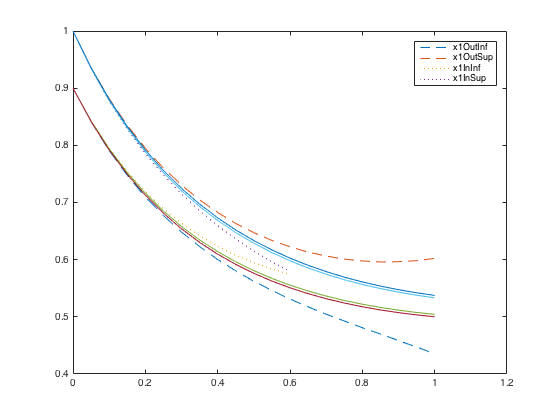
\epsfig{file=brusselator_x1_IA_AA.png,clip=,width=8cm}
\end{center}



The Brusselator (x1): Taylor model of order 4 in t, up to t=10

\begin{center}
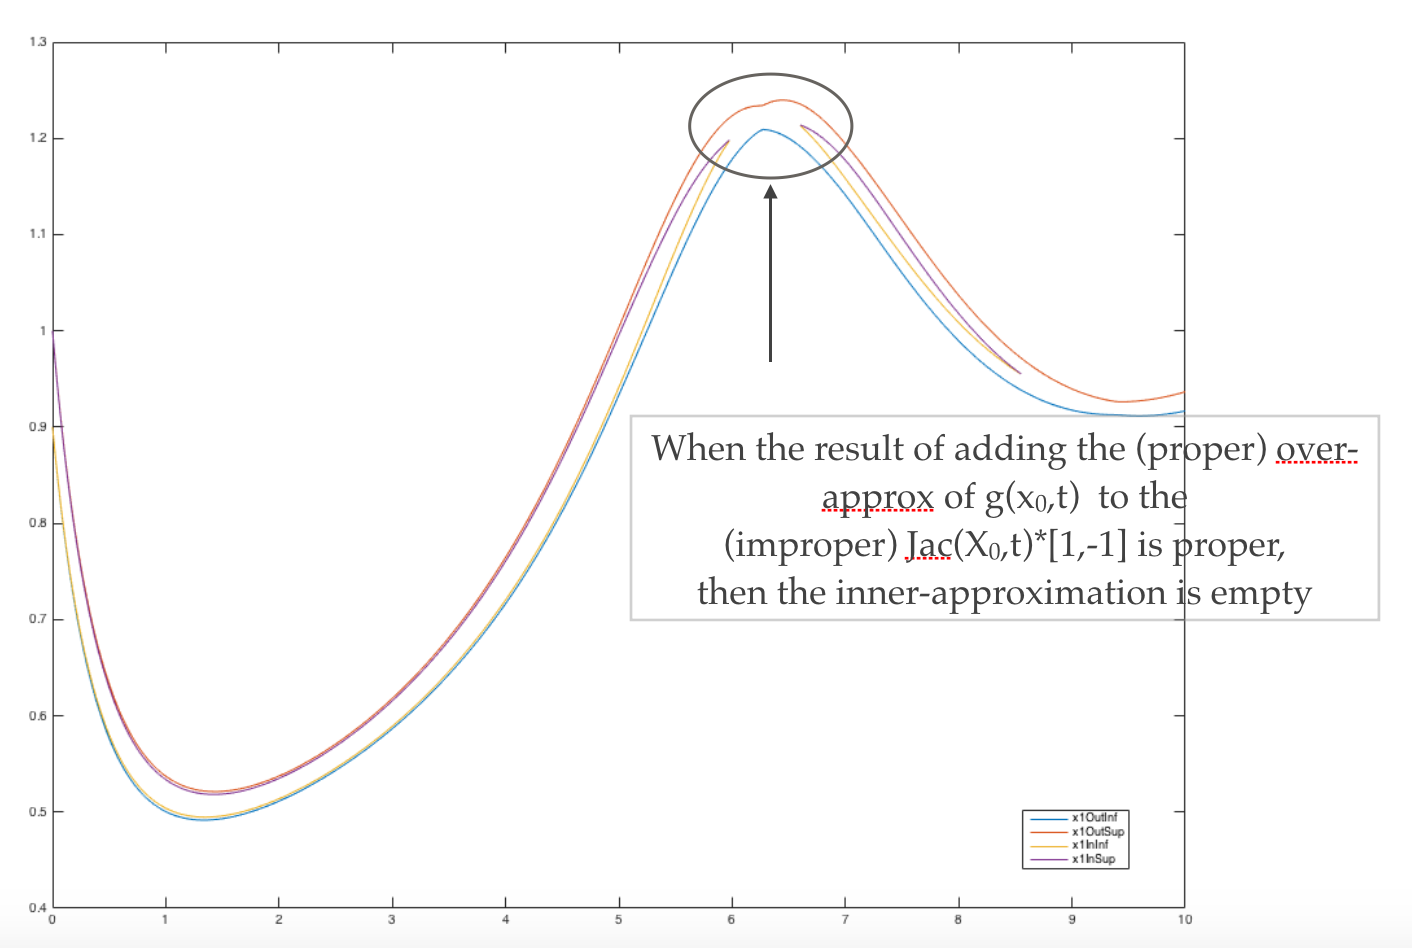
\epsfig{file=brusselator_x1_t10_comment.png,clip=,width=10cm}
% ou version non commentée : 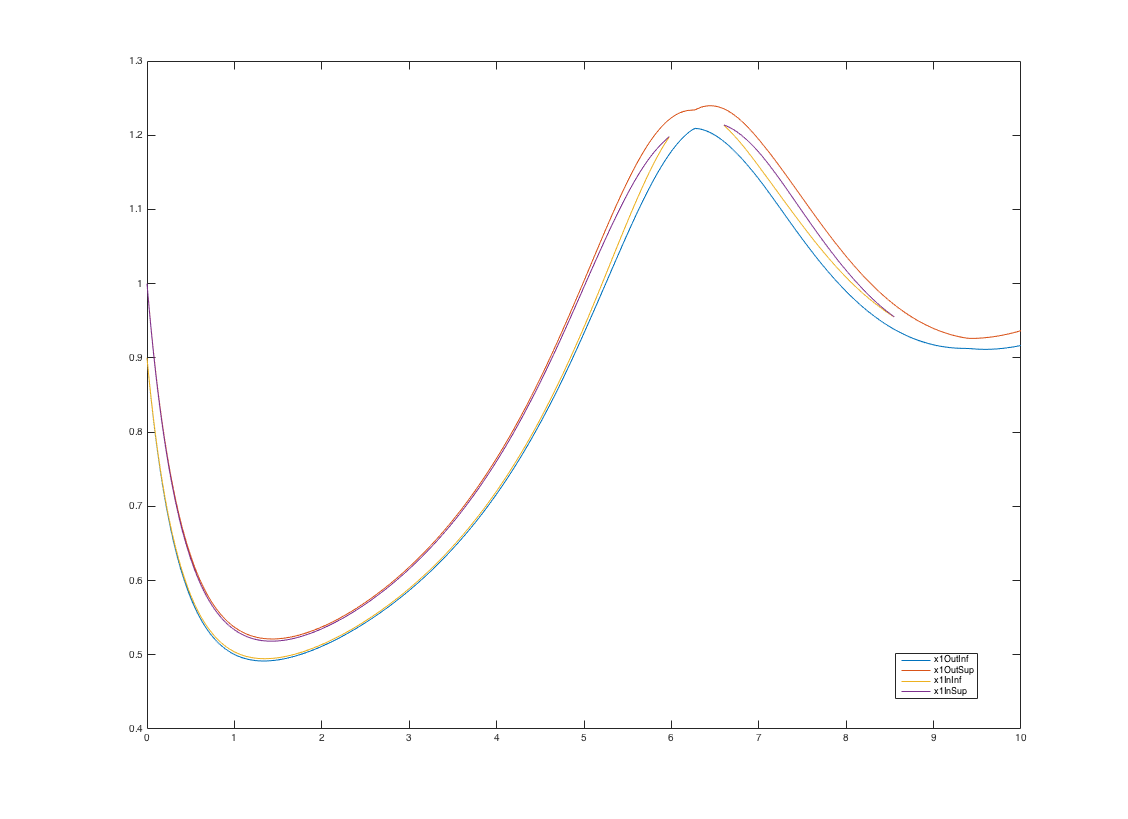
\epsfig{file=brusselator_x1_t10.png,clip=,width=10cm}
\end{center}

The Brusselator (x2): Taylor model of order 4 in t, up to t=10

\begin{center}
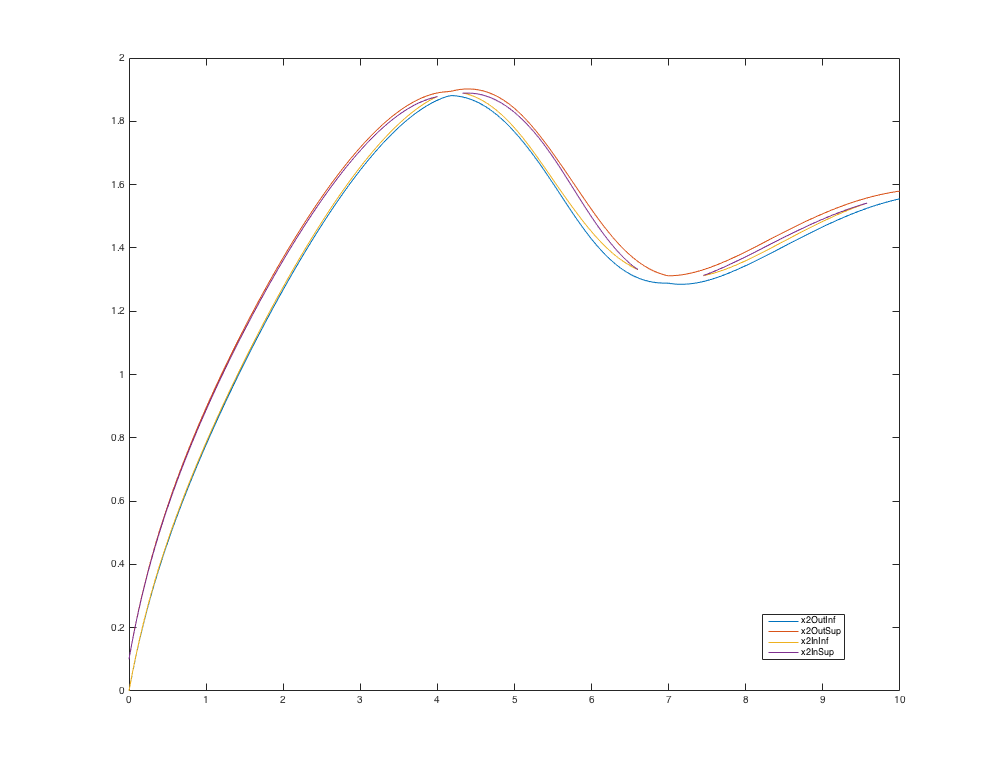
\epsfig{file=brusselator_x2_t10.png,clip=,width=10cm}
\end{center}


\SP{Deja c'est joli - meme si il faudra sans doute que je refasse les figures - commenter que la sous-approx devient vide puis re-apparait, mais aussi reflechir a ce qu'on peut en deduire sur le systeme (cycle?), et si on veut 
que je fasse d'autres experiences}

%------------------------------------------------------------------------------------------------------------------------------------------------

% Exemple retiré car je n'arrive pas a bioen le traiter pour le moment
%\subsection{Car on the hill}
%\[ \left\{ 
%\begin{array}{lll} \dot x_1 & = & x_2 \\
%\dot x_2 & = & - 9.81 \sin(\frac{dg}{dx}(x_1))-0.7 x_2 + u
%\end{array}
%\right.
%\]
%where \[ g(x) = \frac{1}{2} (-\frac{1.1}{1.2} \cos(x) + \frac{1.2}{1.1} cos(1.1x)), \]
%the command $u$ is bounded in $[-2,2]$, the initial condition is $x_1(0) \in [-1,1]$, $x_2(0) \in [-1,1]$, 
%and we have limit conditions $x_1(t) \in [-1,13]$, $x_2(t) \in \R$ (conditions as in T. Le Mezo's document ``viability list of problems'')

%\SP{Si on peut montrer qu'on peut soit reussir a remonter la cite soit rester bloque, un peu comme T. Le Mezo a montre dans sa pres a brest, ca serait chouette. 
%Mais au moins dans l'implem matlab ca explose completement, mais relativement bizarrement: je ne suis qu'a moitié confiante sur l'AA dedans ...}
%}

\subsection{Comparisons to the related work}
\label{sec:exp_compar}
\ForAuthors{To be discussed ;-)}

These benchmarks are taken from \cite{Underapproxflowpipes}. 

\paragraph{Moore-Greitzer model of a jet engine}
\begin{equation}
\dot{\left(\begin{array}{c}
x \\
y
\end{array}\right)} = \left(\begin{array}{c}
-y-1.5x^2-0.5x^3-0.5 \\
3x-y
\end{array}\right)
\end{equation}
The initial set is given by the simplex 
$$X_0=\{(x,y) \in \R^2 | -x \leq -0.9 \wedge -y \leq -0.9\wedge x+y-2 \leq 0\}$$

In \cite{Underapproxflowpipes}, two cases are considered : 
\begin{itemize}
\item computation of the inner and outer approximations of the reachable set at time
$t=0.04$
\item computation of the inner and outer approximations of the reachable set at times
in [0,3] (using a step-size $\delta=0.02$)
\end{itemize}

\ForAuthors{Je rajoute les equations plus tard}

\paragraph{Shimizu-Morioka}

\paragraph{Steam governor}

\paragraph{Biological system}

(also from \cite{underapprox16}?)

\begin{equation}
\dot{\left(\begin{array}{c}
x_1 \\
x_2 \\
x_3 \\
x_4 \\
x_5 \\
x_6 \\
x_7
\end{array}\right)} = \left(\begin{array}{c}
-0.4x_1+5x_3x_4 \\
0.4x_1-x_2 \\
x_2-5x_3x_4 \\
5x_5x_6-5x_3x_4 \\
-5x_5x_6+5x_3x_4 \\
0.5x_7-5x_5x_6 \\
-0.5x_7+5x_5x_6
\end{array}\right)
\end{equation}


\ForAuthors{Les suivants, bof, classiques? mais bien pour benchs si on avait le temps?}

\paragraph{R\"ossler}


\paragraph{Lorenz}

\paragraph{Lotka-Volterra}
(also from \cite{underapprox16}?)

\begin{equation}
\dot{\left(\begin{array}{c}
x_1 \\
x_2 \\
x_3
\end{array}\right)} = \left(\begin{array}{c}
x_1x_2-x_1x_3 \\
x_2x_3-x_2x_1 \\
x_3x_1-x_3x_2
\end{array}\right)
\end{equation}

\paragraph{Coupled Van der Pol}

The next set of examples is taken from \cite{underapprox16}. 

\paragraph{Electromechanical oscillation}

\begin{equation}
\dot{\left(\begin{array}{c}
x \\
y
\end{array}\right)} = \left(\begin{array}{c}
y \\
0.2-0.7sin(x)-0.05y
\end{array}\right)
\end{equation}
The initial set is given by $[-0.1,0.1]\times [2.9,3.1]$. We are looking at an 
inner-approximation at times $t=0.5$ and $t=3$. 

\paragraph{Van der Pol}

\begin{equation}
\dot{\left(\begin{array}{c}
x_1 \\
x_2
\end{array}\right)} = \left(\begin{array}{c}
x_2 \\
-0.2(x^2_1-1)x_2-x_1
\end{array}\right)
\end{equation}

%------------------------------------------------------------------------------------------------------------------------------------------------

%******************************************************************************
\section{Conclusion and future work}
%******************************************************************************
%
\begin{itemize}
\item Hybrid systems (and inner-approximated constraints)
\item combination with backward inner-approximated analyses ? 
\item abstract model-checking ? 
\end{itemize}

\bibliographystyle{abbrv}
\bibliography{hscc2017}

\end{document}
